\documentclass{article}

\newcommand{\rnum}[1]{\uppercase\expandafter{\romannumeral #1\relax}}

\usepackage[utf8]{inputenc}
\usepackage[T1]{fontenc}
\usepackage[ngerman]{babel}
\usepackage[margin=2.5cm]{geometry}
\usepackage{graphicx}
\usepackage{float}

\begin{document}

\begin{titlepage}
	{
		\centering
		\huge
		\textbf{Abgabedokument Prozess}\\
	}
	\vspace{1cm}
	\begin{table}[h]
		\centering
		\footnotesize
		\begin{tabular}{| p{1.5cm} | p{2.5cm} | p{2cm} | p{2cm} | p{2cm} |}
			\hline
			                           & Verantwortliche Teammitglieder (Organisation, Anlegen der Dokumentenversion, Moderation, Abgabe)                                   & Anwesende während der Meetings                                                                                                     & (Online-) Beiträge zum Inhalt durch                                                                                                & Korrektur-gelesen durch                                                                                                            \\
			\hline
			Dokument Prozess Version 1 & Paul Schröder, Eric Buthmann, Yanik Buthmann, Erik Seeck, Mathis Behrendt, David Nguyen, Adrian Gode, Niklas Krüger, Kevin Zellmer & Paul Schröder, Eric Buthmann, Yanik Buthmann, Erik Seeck, Mathis Behrendt, David Nguyen, Adrian Gode, Niklas Krüger, Kevin Zellmer & Paul Schröder, Eric Buthmann, Yanik Buthmann, Erik Seeck, Mathis Behrendt, David Nguyen, Adrian Gode, Niklas Krüger, Kevin Zellmer & Paul Schröder, Eric Buthmann, Yanik Buthmann, Erik Seeck, Mathis Behrendt, David Nguyen, Adrian Gode, Niklas Krüger, Kevin Zellmer \\
			\hline
			Dokument Prozess Version 2 & Paul Schröder, Eric Buthmann, Yanik Buthmann, Erik Seeck, Mathis Behrendt, David Nguyen, Adrian Gode, Niklas Krüger, Kevin Zellmer & Paul Schröder, Eric Buthmann, Yanik Buthmann, Erik Seeck, Mathis Behrendt, David Nguyen, Adrian Gode, Niklas Krüger, Kevin Zellmer & Paul Schröder, Eric Buthmann, Yanik Buthmann, Erik Seeck, Mathis Behrendt, David Nguyen, Adrian Gode, Niklas Krüger, Kevin Zellmer & Paul Schröder, Eric Buthmann, Yanik Buthmann, Erik Seeck, Mathis Behrendt, David Nguyen, Adrian Gode, Niklas Krüger, Kevin Zellmer \\
			\hline
		\end{tabular}
	\end{table}
\end{titlepage}

\section{Reflektion Lego Workshop \rnum{1}}
Die Aufgabe bestand darin, eine Stadt aus Klemmbausteinen zu bauen.
Ein Stakeholder formulierte Anforderungen an die Stadt, die unterschiedlich priorisiert waren, und grenzte die Arbeitszeit ein.
Die Bewältigung dieser Aufgabe sollte eine Gruppe, bestehend aus ungefähr 30 Personen, übernehmen.\\
Nach der Bekanntgabe der Aufgabe, bildete sich eine kleine Gruppe, welche die Führung übernahm.
Diese Gruppe begann dann, die Anforderungen der Gruppe vorzulesen.
Nach dem Vorlesen der Anforderungen wurde zunächst die Größe der gesamten Gruppe ermittelt.
Die gesamte Gruppe wurde daraufhin in kleine Gruppe von jeweils etwa 5 Personen aufgeteilt.
Daraufhin bekamen die meisten Gruppen einen Verantwortungsbereich, wie zum Beispiel dem Bau von Wohnhäusern, zugeteilt.
Eine Gruppe bekam die Aufgabe das Gesamtbild der Stadt zu planen.
Bei der Durchführung bauten dann die kleinen Gruppen die benötigten Bestandteile der Stadt.
Das Führungsteam führte eine Liste mit den bereits erfüllten Anforderungen und koordinierte die weitere Aufgabenverteilung.
Zum Ende der vorgegebenen Zeit wurden die einzelnen Bestandteile der Stadt, so wie es die zuständige Gruppe geplant hat, zusammengeführt.\\
Abschließend wurde das Ergebnis mit dem Stakeholder zusammen beurteilt.\\
\\
Bei der Bearbeitung der Aufgabe gab es einige Vorgehensweisen, die in Zukunft beibehalten werden können.
In kurzer Zeit hat eine kleinere Gruppe die Führung der restlichen Gruppe übernommen.
So konnten zeitnah Entscheidungen über den weiteren Projektverlauf getroffen werden.
Die Aufteilung in kleinere Gruppen mit eigenen Zuständigkeitsbereichen war ebenfalls von Vorteil.
Dadurch konnten mehrere Anforderungen parallel bearbeitet werden und die Kommunikation in diesen Gruppen war einfacher, als in einer großen Gruppe.
Als hilfreich erwies sich die Gruppe, welche die Planung des Gesamtbildes der Stadt als Sonderaufgabe übernahm.
Die aufgestellten Richtlinien trugen dazu bei, dass am Ende alle Komponenten der Stadt zusammenpassten.
Die Anforderungen des Stakeholders wurden außerdem vereinzelt hinterfragt und der Stakeholder wurde um eine genauere Spezifizierung gebeten.
Dies erleichterte den Bauprozess und führte am Ende zu einem Ergebnis, welches näher an den Vorstellungen des Stakeholders lag.
Abschließend ist hervorzuheben, dass die fertiggestellten Anforderungen von der Führungsgruppe gesammelt wurden.
Eine Folge dessen war ein besserer Überblick über die Gesamtsituation des Stadtbaus.
Bisher fehlende Komponenten konnten so identifiziert und deligiert werden.\\
\\
Einige Vorgehensweisen führten jedoch zu Problemen, die das Ergebnis negativ beeinflussten.
Zum einen war die Größe der Arbeitsgruppen zu groß.
Eine Gruppe, welches für den Bau von einem Haus vorgesehen war, sollte aus fünf Personen bestehen.
Diese Größe war nicht effizient, da nur zwei Personen gleichzeitig an einem Haus bauen konnten.
Die restlichen Gruppenmitglieder hatten dann Leerlauf.
Zum anderen wurden keine zeitlichen Einschränkungen für das Erledigen von Aufgaben festgelegt.
Das führte dazu, dass die Gruppen bis zum Ablauf der Zeit an ihrer initial zugteilten Aufgaben arbeiteten und keine weiteren benötigten Anforderungen bearbeitet werden konnten.
Desweiteren fielen einige Unstimmigkeiten aufgrund zu allgemein formulierter Anforderungen auf.
Bei der Abnahme durch den Stakeholder wurde unter anderem deutlich, dass die Anzahl der Wohnhäuser zu gering war und einige Komponenten anders gebaut wurden, als ursprünglich vom Stakeholder gemeint.
Außerdem bemängelte der Stakeholder, dass einige Anforderungen, welche eine hohe Priorisierung besaßen, nicht erfüllt wurden.
Ein Grund dafür kann die in einem nicht ausreichenden Maße durchgeführte Anforderungsüberwachung sein.
Es wurde begonnen, die erledigten Aufgaben zu sammeln.
Einige Arbeitsgruppen bekamen dies jedoch nicht mit und behielten die Anforderungszettel, sodass der Überblick über die zu erledigenden Aufgaben und die zur Verfügung stehenden Gruppen verloren ging.
Abschließend negativ aufgefallen ist, dass jegliche Qualitätssicherung fehlte.\\
\\
In einer zukünftigen Ausführung der Aufgabe kann man nun folgende Verbesserungen vornehmen:
\begin{enumerate}
	\item Die Gruppengröße wird verringert.
	\item Jede Gruppe holt sich zu Beginn der Arbeitszeit eine Anforderung von der Führungsgruppe, welche einen zeitlichen Rahmen festlegt.
	      Nach Fertigstellung der Anforderung wird der Zettel der Anforderung an die Führungsgruppe zurückgegeben und es wird eine neue Anforderung geholt.
	\item Die Führungsgruppe führt eine Übersicht über die erledigten Anforderungen und plant je nach Priorisierung, was als nächstes erledigt werden muss.
	\item Bei Unklarheiten bezüglich einer Anforderung, befragt die Arbeitsgruppe den Stakeholder.
	\item Es werden Qualitätsanforderungen definiert und es wird eine Gruppe gegründet, welche diese während der gesamten Arbeitszeit überwacht.
\end{enumerate}

\begin{figure}[H]
	\centering
	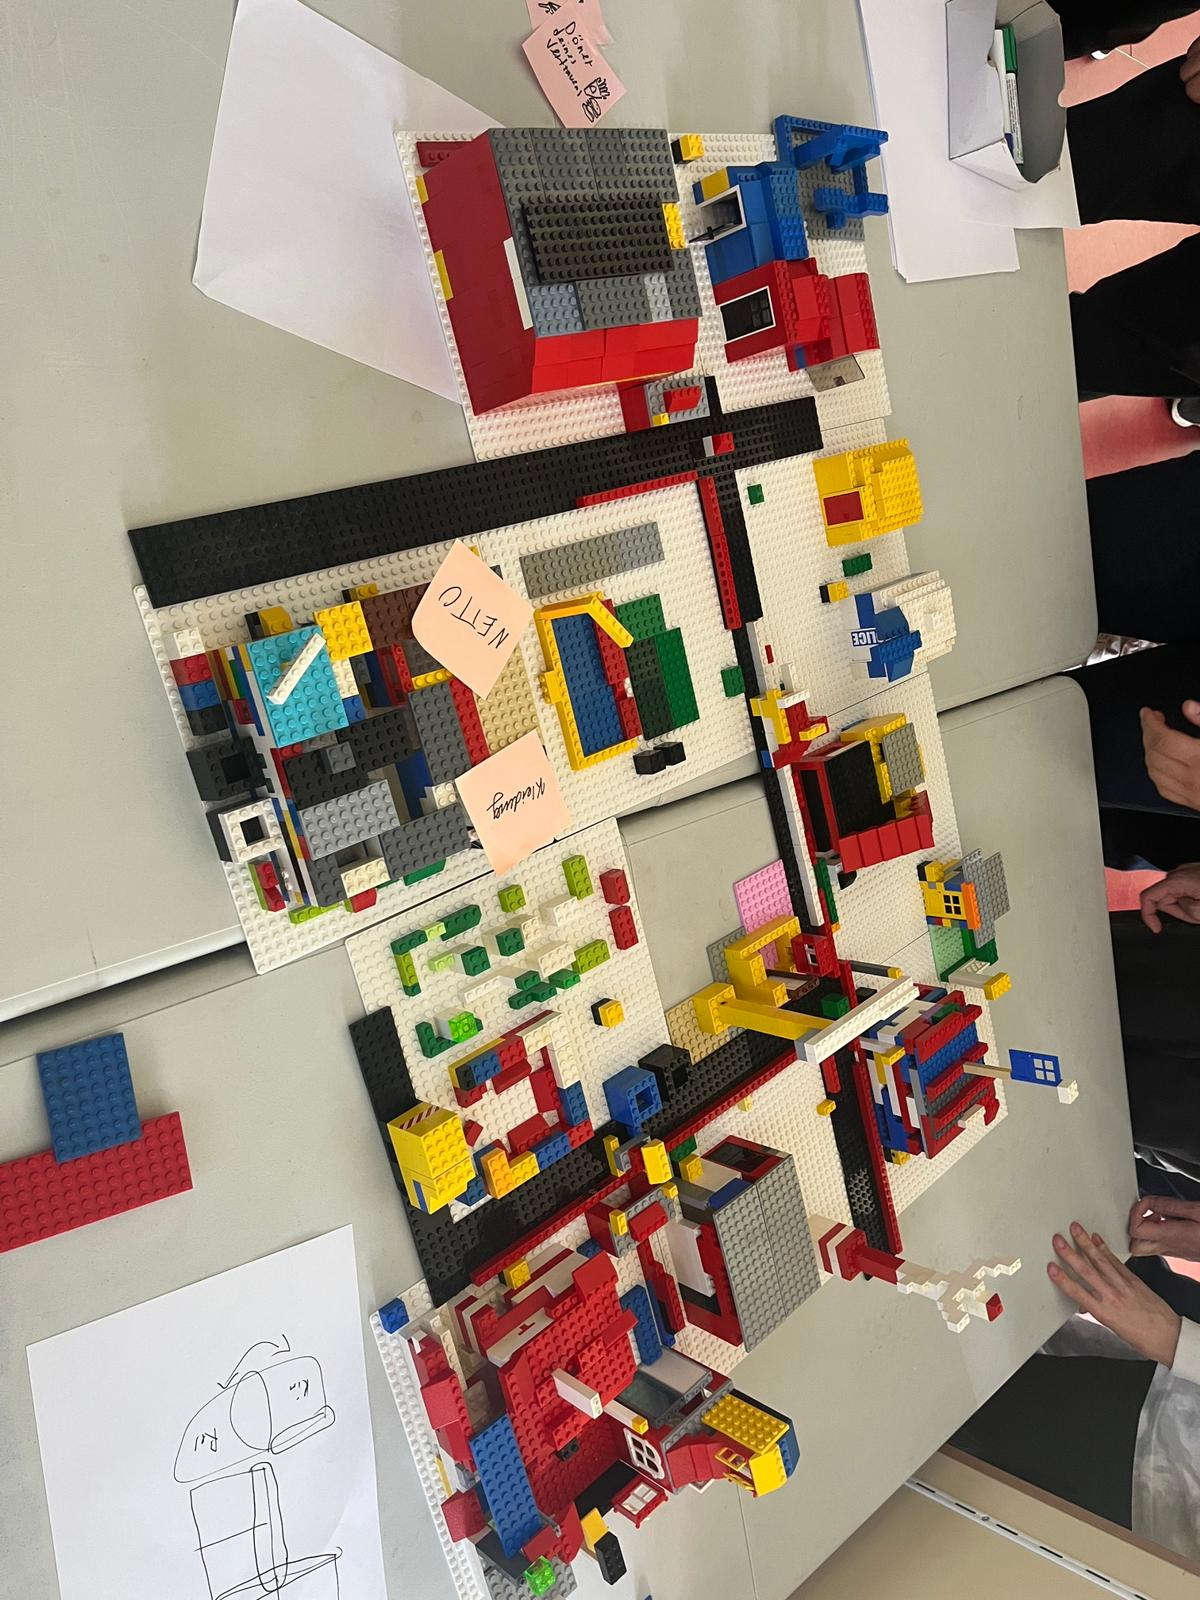
\includegraphics[width=0.6\textwidth, angle=90]{stadt.jpg}
	\caption{Foto der gebauten Stadt im zweiten Workshop}
\end{figure}

\newpage

\section{Reflektion Lego Workshop \rnum{2}}

Im zweiten Lego Workshop lag der Fokus auf dem Bau eines Hafens. Genau wie beim
ersten Workshop meldete sich wieder eine kleine Gruppe freiwillig dafür, die
Leitung zu übernehmen. Darunter ließ sich besonders eine Person als eine Art
Projektmanager ausmachen. Anders war dieses Mal jedoch, dass wir nach dem
\textit{Scrum-of-Scrums}-Prinzip arbeiteten. Die gesamte Gruppe wurde in kleinere
Teams aufgeteilt, die jeweils konkrete Aufgaben übernahmen. Die Aufteilung erfolgte
den Projektteams entsprechend, wodurch die Teamgrößen bei 6-8 Personen lagen.
Die leitende Gruppe koordinierte die Arbeit der Teams, indem sie einige User
Stories und Requirements zusammenfasste und diese an die Teams verteilte. So
war jedes Team für einen bestimmten Bereich des Hafens verantwortlich, wie zum
Beispiel den Bau von Docks, bestimmten Häusern, Kränen oder der Belichtung.

Verglichen mit dem ersten Workshop zeigte sich bereits an dieser Stelle eine deutliche Verbesserung:
Während im Stadtbau-Workshop viele Entscheidungen spontan und teilweise chaotisch getroffen wurden, sorgte die Aufteilung in feste Teams mit klaren Zuständigkeiten im zweiten Workshop für mehr Struktur und Transparenz. Die Rollen waren klarer verteilt, und im Gegensatz zum ersten Workshop wusste jedes Team jederzeit, an welcher Aufgabe es arbeitete und wie diese in das Gesamtbild passte.

Unsere eigenen Aufgaben umfassten zunächst den Bau von Laternen, Scheinwerfern
und einem Aussichtsturm. Für die darauffolgenden zwei Iterationen waren jeweils
8 Minuten zur Planung, 8 Minuten für den Bau und 8 Minuten Retrospektive
vorgegeben. In unserem 6-köpfigen Team verteilten wir die Aufgaben zunächst auf
2 Unterteams. Ein Unterteam übernahm den Bau der Laternen und Scheinwerfer, während
das andere Team den Aussichtsturm konzipierte und baute. Zum Ende der Iteration waren unsere Teamaufgaben fast abgeschlossen, woraufhin wir die Retrospektive durchführten.
Nach dem anschließenden Scrum-of-Scrums-Meeting wurden neue Aufgaben verteilt, darunter
der Bau einer Zollstation und eines kleinen Gebäudes für die Hafenmitarbeiter.
Erneut teilten wir in der Planungsphase die Aufgaben in unseren Unterteams auf,
besprachen Design und Vorgehen und begannen mit dem Bau.
Wir schlossen unsere Aufgaben innerhalb der vorgegebenen Zeit ab und setzten zuletzt
die gebauten Komponenten in den Hafen ein, dessen Layout vom leitenden Team geplant wurde.

Die Anwendung der Scrum-of-Scrums-Methode erwies sich als besonders hilfreich für
die Koordination mehrerer Teams. Die Meetings ermöglichten
es, den Fortschritt zu überprüfen, auftretende Probleme frühzeitig zu identifizieren
und Aufgaben neu zu priorisieren. Dadurch konnten alle Teams fokussiert an ihren
Aufgaben arbeiten, ohne dass es zu Überschneidungen kam oder man sich Gedanken
über das Fertigstellen anderer Komponenten machen musste. Außerdem erleichterte
die klare Aufteilung der Aufgaben die Verantwortung jedes Teams: Jeder wusste
genau, für welchen Teil des Hafens er zuständig war.

Auch hier zeigte sich ein großer Fortschritt gegenüber dem ersten Workshop:
Dort ging häufig der Überblick verloren, welche Gruppen bereits Anforderungen erfüllt hatten oder wo Engpässe bestanden. Im zweiten Workshop hingegen sorgten die regelmäßigen Abstimmungspunkte dafür, dass Informationen gezielt zwischen den Teams flossen, statt - wie beim ersten Mal - zufällig oder verzögert durch einzelne Personen. Dies führte zu einem flüssigeren Arbeitsprozess und weniger Missverständnissen.

Ein weiterer positiver Aspekt war die Möglichkeit, kreative Lösungen innerhalb
der eigenen Aufgaben zu entwickeln. Beispielsweise konnten wir beim Bau der
Laternen und Scheinwerfer unterschiedliche Designs ausprobieren.

Des Weiteren war die Arbeitsweise unseres Teams durch das Aufteilen in kleinere
Gruppen besonders effektiv. So konnte jedes Unterteam parallel an seinen Aufgaben arbeiten, ohne
dass Personen Leerlauf hatten. Somit erwies sich insbesondere die Zeit zum Planen
in den Teams als hilfreich. Auch das Meeting mit dem Stakeholder zwischen den
beiden Iterationen half dabei, die Anforderungen besser zu verstehen und
sicherzustellen, dass die gebauten Komponenten den Erwartungen entsprachen.
So konnten wir uns nach dem Feedback an unseren Komponenten sicher sein, dass
wir auf dem richtigen Weg waren.

Im direkten Vergleich zum ersten Workshop war auch der Umgang mit Anforderungen deutlich flexibler und effektiver.
Während die Teams beim Stadtbau-Workshop oft bis zum Ende an ihren initialen Aufgaben festhielten - selbst wenn sich Prioritäten verschoben - erlaubte die iterative Vorgehensweise im zweiten Workshop ein rechtzeitiges Umlenken. Neue Anforderungen konnten aufgenommen, unpassende Designideen früh korrigiert und der Arbeitsumfang realistischer eingeschätzt werden.

Trotz der verbesserten Organisation gab es noch einige Verbesserungspotenziale.
Insbesondere hörte man in der abschließenden Feedbackrunde, dass einige Teams
die Teamgrößen als zu groß empfanden. Dies führte dazu, dass nicht alle Teammitglieder
gleichermaßen aktiv am Bauprozess beteiligt waren. Wir kamen zu dem Schluss, dass
bei der Teamgröße und der Art von Aufgaben ein weiteres Scrum-of-Scrums-Prinzip
innerhalb der Teams sinnvoll gewesen wäre. Des Weiteren wurde bemängelt, dass die
Zeit für die Planung und Retrospektive im Verhältnis zur Bauzeit zu lang war. Die
Planung war so auch in unserem Team recht schnell beendet, und es wurde mehr oder
weniger nur noch auf den Baubeginn gewartet.

Obwohl unser Projektmanager eine wirklich gute Arbeit bei der Koordination der Teams
leistete und einem das Gefühl vermittelte, dass er wusste, was er tat, gab es Kritik
hinsichtlich der Übersicht über den aktuellen Stand der einzelnen Teams. Insbesondere
wäre es vermutlich schwer gewesen, auf Fragen des Stakeholders während einer
Iteration einzugehen und Auskünfte über den Fortschritt der einzelnen Teams und
Komponenten zu geben.

Abschließend lässt sich sagen, dass der zweite Workshop deutlich erfolgreicher verlief als der erste. Die Arbeit nach dem Scrum-of-Scrums-Prinzip sowie die Aufteilung in kleinere Teams führten zu einer besseren Organisation und effizienteren Bearbeitung der Aufgaben. Die zusätzlichen Meetings und Iterationen ermöglichten eine engere Abstimmung zwischen den Teams und verbesserten die Kommunikation. Gleichzeitig zeigte sich, dass die Zeitverteilung noch optimiert werden könnte: Mehr Zeit sollte für den Bau der Komponenten und weniger für Planung und Retrospektive eingeplant werden.
Darüber hinaus wäre die Einführung eines Backlogs mit klaren Statusangaben wie „Todo“, „In Progress“
und „Done“ sinnvoll gewesen, um den Überblick über die Aufgaben und deren Fortschritt zu behalten.

Auch wenn der zweite Workshop damit deutlich strukturierter und erfolgreicher war als der erste, zeigte der Vergleich beider Durchläufe sehr gut, wie wichtig klare Rollen, definierte Kommunikationswege und ein iteratives Vorgehen sind. Viele der Probleme des ersten Workshops - etwa unklare Zuständigkeiten, fehlende Priorisierung oder unübersichtliche Anforderungslisten - konnten durch das Scrum-of-Scrums-Prinzip weitgehend vermieden werden. Gleichzeitig wurde sichtbar, wo noch Potenzial besteht, um den Ablauf weiter zu verbessern.

\begin{figure}[H]
	\centering
	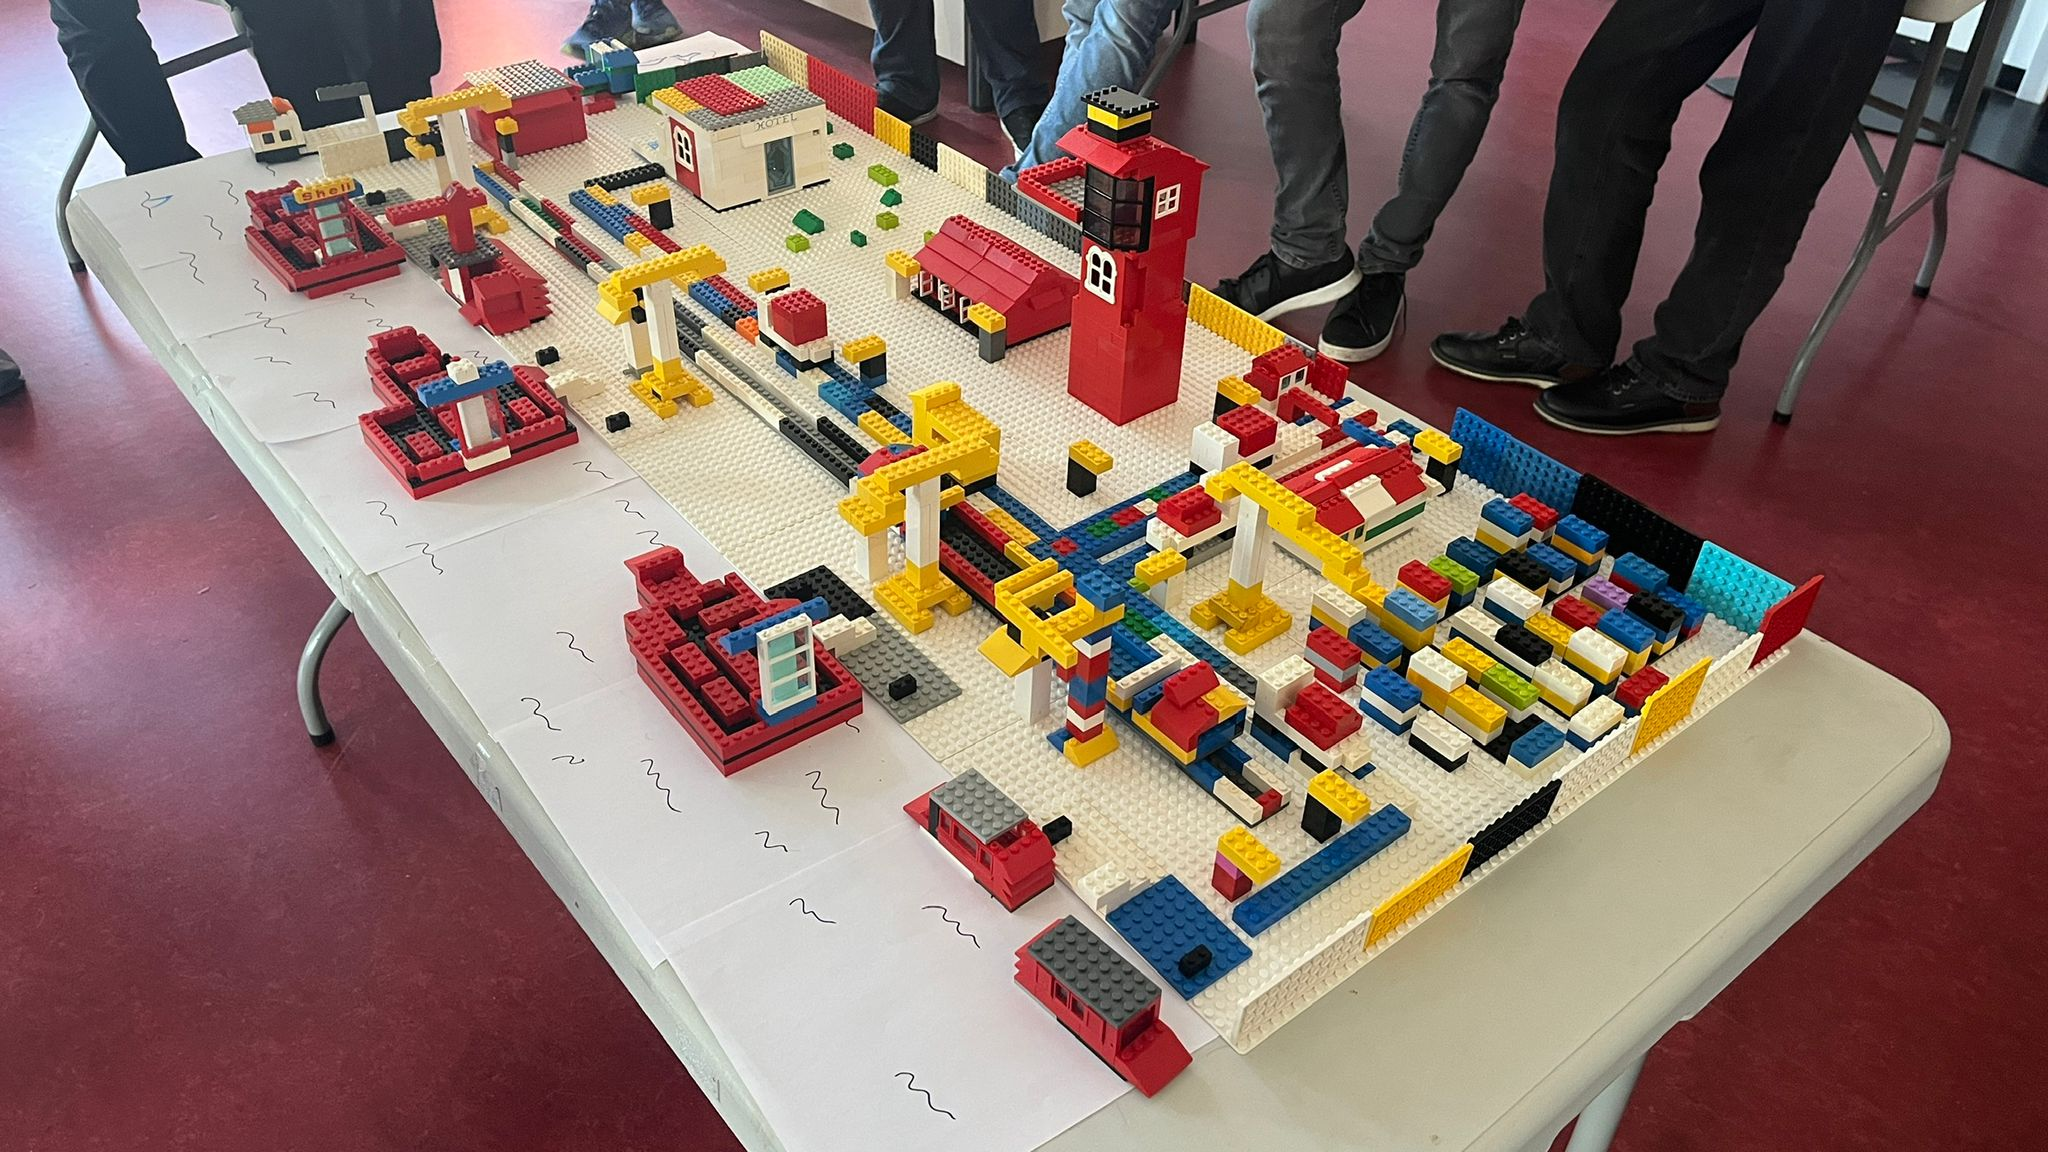
\includegraphics[width=0.8\textwidth]{hafen.jpg}
	\caption{Foto des gebauten Hafens im zweiten Workshop}
\end{figure}

\section{Prozessplan}

\subsection{Rollen}
Für die Durchführung des Projektes erachten wir die Vergabe der Rollen Prodcut Owner, Scrum Master und Entwickler als sinnvoll.

\subsubsection{Product Owner}
Der Product Owner ist dafür zuständig, ein Überblick über das Backlog zu behalten.
Zum Beginn eines Sprints definiert dieser, welche Anforderungen mit welcher Priorität implementiert werden sollen.\\
Außerdem ist der Product Owner der Ansprechpartner für die Entwickler, wenn diese Verständnisprobleme bei zugewiesenen Anforderungen haben.
Sollte auch der Product Owner Anforderungen nicht verstehen, dann ist dieser dafür zuständig, die Unklarheiten mit einem Stakeholder zu klären.\\
Da der Umfang der Aufgaben eines Product Owners in diesem Projekt überschaubar ist, kann ein Product Owner auch gleichzeitig die Rolle eines Entwicklers einnehmen.\\
Die Rolle des Product Owners wird zu jedem Sprint neu besetzt, um eine faire Aufteilung der Arbeit zu gewährleisten.\\
Wir haben uns für die Besetzung der Rolle des Product Owners entschieden, damit es nur eine Person gibt, die Unklarheiten mit dem Stakeholder bespricht.\\
Ein Nachteil dieser Entscheidung ist, dass der aktuelle Product Owner zwei Rollen einnimmt und so von einer höheren Belastung betroffen ist.
In zukünftigen Sprints kann man daher die Rolle des Product Owners als vollwertige Rolle betrachten und der betroffenen Person keine Entwicklungsaufgaben zuteilen.

\subsubsection{Scrum Master}
Der Scrum Master sorgt dafür, dass das Scrum-Framework richtig eingesetzt wird.
Hierfür plant dieser die Teammeetings, moderiert diese und sorgt dafür, dass die Meetings produktiv durchgeführt werden.
Außerdem bereitet der Scrum Master das Feedback des Projektteams zum Ende des Sprints auf und trifft Vorbereitungen für einen optimierten nächsten Sprint.\\
Für den Scrum Master gilt ebenfalls, dass dieser auch die Rolle des Entwicklers einnehmen kann.
Dies hat den Hintergrund, dass in einem kleinen Projekt ein Scrum Master nur wenige Aufgaben besitzt und zusätzliche Kapazität zu Verfügung hat.\\
Die Rolle des Scrum Masters wird analog zum Product Owner zu jedem Srint neu besetzt.\\
Für die Vergabe der Rolle des Scrum Masters haben wir uns entschieden, weil eine Scrum Master die Produktivität in einem Projektteam fördert und die Einhaltung der Richtlinien überwacht.\\
Der Scrum Master wird ebenfalls höher belastet.
Sollte der Aufwand als Scrum Master und Entwickler zu hoch werden, werden wir im nächsten Sprint einen dedizierten Scrum Master einführen.

\subsubsection{Entwickler}
Ein Entwickler hat in unserem Projektteam mehrere Aufgaben.\\
Zu Beginn eines Sprints bekommt dieser eine oder mehrere Anforderungen zugeteilt.
Aus der Definition der Anforderungen muss der Entwickler dann ausführbare Aufgaben ableiten.
Bei Unklarkeiten oder Verständnisproblemen hat ein Entwickler die Möglichkeit, den Product Owner um Hilfe zu bitten.\\
Nach der Ableitung der Aufgaben beginnt der Entwickler mit der Planung der Umsetzung.
Hierbei erstellt dieser notwendige Diagramme und prüft, ob Schnittstellen zu anderen Teilen des Systems benötigt werden.
Ist dies der Fall hat der Entwickler die Möglichkeit, andere Entwickler, welche aktuell an dem betroffenen Teil des Systems arbeiten, zu konsultieren und notwendige Absprachen zu treffen.\\
Nach erfolgter Planung beginnt der Entwickler mit der Implementierung.
Sollte für die Implementierung zusätzliches Wissen benötigt werden, kann der Entwickler selbstständig Zeit für eine Weiterbildung einplanen.\\
Für die Qualitätssicherung ist ebenfalls der Entwickler zuständig.
Hierfür muss der Entwickler automatisierte Tests erstellen und die gesamtheitliche Korrektheit des Systems manuell überprüfen.\\
Nach der Implementierung hat ein Entwickler eine angemessene Dokumentation der Erweiterung zu erstellen.\\
In unserem Projektteam übernimmt ein Entwickler somit die Aufgaben eines Anforderungsanalytikers, eines Architekts, eines Testers und logischerweise eines Entwicklers.
Dies hat den Vorteil, dass ein Entwickler größtenteils autonom arbeiten kann und nicht auf die Zuarbeit von anderen Projektmitgliedern angewiesen ist.\\
Allerdings hat ein Entwickler damit viele Aufgaben zu erledigen und kann sich nur geringfügig spezialisieren.
Der Vorteil von dedizierten Architekten wäre zum Beispiel, dass diese sich auf die Architektur des Systems spezialisieren können und so in darauffolgenden Sprints eine höhere Arbeitsgeschwindigkeit hätten.\\
Sollte sich der Aufwand für einen Entwickler als zu hoch erweisen, können in folgenden Sprints zusätzliche Rollen definiert werden.

\end{document}
